\subsection{Closed Form Expressions of Quantities for the General $2\times 2$ Spin Case}
\label{sec:ClosedFormSolution}
The system consisting of $2\times 2$ spins has in total $2^4 = 16$ spin configurations. 
These $16$ configurations are given in \figref{fig:SpinConfigurations} below. 
\begin{figure}[H]
	\centering
	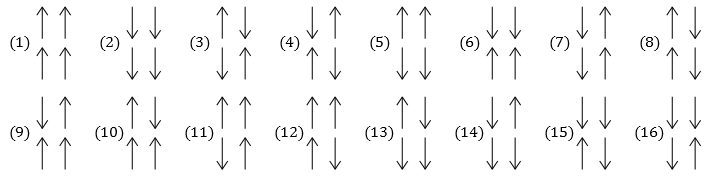
\includegraphics[width=0.75\textwidth]{Figures/Configurations.png}
	\caption{The 16 different spin configurations for the 2 dimensional case with 2 spins in each dimension. An arrow pointing upwards represents spin up with the spin value $s_{up}=+1$, whilst an arrow pointing downwards represent spin down with the spin value $s_{down}=-1$. The corresponding energies and magnetizations of each of the micro states can be found in \tabref{tab:ClosedFormSolution1}.}
	\label{fig:SpinConfigurations}
\end{figure}
The energy and magnetization for each of the $16$ microstates are given in \tabref{tab:ClosedFormSolution1} and are calculated from \matref{eq:EnergyMagnetization}. 
As an example, the energy and magnetization of the ninth microstate, given in \figref{fig:SpinConfigurations} as the state with one spin down and three spin up, is calculates here:
\begin{align*}
	E_9 &= -J \sum_{<kl>} ^{2\times 2} s_k s_l
	\\
	&= -J[((-1)\cdot 1 + (-1) \cdot 1)+(1\cdot (-1) + 1\cdot 1) + (1\cdot (-1) + 1\cdot 1 ) +(1\cdot 1 + 1\cdot 1)]
	\\
	&= 0
\end{align*}
and
\begin{align*}
	\mathcal{M} _9 = \sum _{j=1} ^{2\times 2} s_j = (-1) + 1 + 1 + 1 = 2
\end{align*}
\begin{table}[H]
\centering
\caption{Energy and magnetization of each of the spin configurations given in \figref{fig:SpinConfigurations}.}
\begin{center}
\begin{tabular}{ |l | c | c | }
  \hline			
  Configuration & Energy & Magnetization  \\
  \hline
  (1) & $-8J$ & $4$ \\
  \hline
  (2) & $-8J$ & $-4$ \\
  \hline
  (3) -- (4) & $8J$ & $0$ \\
  \hline
  (5) -- (8) & $0$ & $0$ \\
  \hline
  (9) -- (12) & $0$ & $2$ \\
  \hline
  (13) -- (16) & $0$ & $-2$ \\
  \hline
\end{tabular}
\end{center}
\label{tab:ClosedFormSolution1}
\end{table}
Hence the partition function $Z$ defined in \matref{eq:PartitionFunction} for this $2\times 2$ spin system becomes
\begin{align}
	Z = 12 + 2\left( e^{8\beta J} + e^{-8 \beta J} \right)
	= 12 + 4\cosh (8\beta J)
	\label{eq:PartitionFunction2times2}
\end{align}
In the last equation sign, Euler's identity \fxnote{ok?} and the definition of $\cosh \theta$ is used.
With this partition function and the energy and magnetization for each of the $16$ microstates given in \tabref{tab:ClosedFormSolution1}, the expectation value of the energy and the magnetization becomes
\begin{align}
	\left< E \right> = \frac{1}{Z} (-16 J e^{8\beta J} + 16 J e^{-8\beta J} )
	 = \frac{16J}{Z} (e^{-8\beta J}-e^{8\beta J})
	 \label{eq:ExpectationEnergy2times2}
\end{align} 
and
\begin{align}
	\left< \mathcal{M} \right> = \frac{1}{Z} (4e^{8\beta J} -4e^{8\beta J} +2 -2 ) = 0 
	\label{eq:ExpectationMagnetization2times2}
\end{align}
However, the expectation value of the absolute value of the magnetization differ from zero. 
That is
\begin{align}
	\left< | \mathcal{M} | \right> = \frac{1}{Z} \left( |4|e^{8\beta J} + |-4|e^{8\beta J} +|2| + |-2| \right) = 
	\frac{1}{Z} ( 8 e^{8\beta J} + 4 ) 
\end{align}
To compute the specific heat $C_v$ and the susceptibility, the quantities $\left< E^2 \right>$ and $\left< \mathcal{M}^2 \right>$ must be known.
For this $2\times 2$ spin case they become
\begin{align}
	\left< E^2 \right> = \frac{1}{Z} \sum _{i=1} ^{16} E_i ^2 e^{-\beta E_i}
	= \frac{128 J^2}{Z} (e^{8\beta J} + e^{-8\beta J} ) 
	\label{eq:ExpectationEnergySquared2times2}
\end{align}
and 
\begin{align}
	\left< \mathcal{M}^2 \right> = \frac{1}{Z} \sum _{i=1} ^{16} \mathcal{M}_i ^2 e^{\beta E_i}
	= \frac{32}{Z} (e^{8\beta J} + 1 ) 
	\label{eq:ExpectationMagnetizationSquared2times2}
\end{align}
The specific heat $C_v$ and the susceptibility $\chi$ can now be determined by the expressions in \matref{eq:SpecificHeatSusceptibility}, and after some joggling with the results gained by \matref{eq:ExpectationEnergy2times2}, \eqref{eq:ExpectationMagnetization2times2}, \eqref{eq:ExpectationEnergySquared2times2} and \eqref{eq:ExpectationMagnetizationSquared2times2}, it is evident that
\begin{align}
	C_v = \frac{128 J^2}{Z k_B T^2} \left[ e^{8\beta J} + e^{-8\beta J} - \frac{2e^{-16\beta J}+2e^{16\beta J}+4}{Z} \right]
	\label{eq:SpecificHeat2times2}
\end{align}
\fxnote{check that this is correct}
and
\begin{align}
	\chi = \frac{1}{k_B T Z} \left[ 32(e^{8\beta J} +1) - \frac{1}{Z}\left( 8e^{8\beta J} +4 \right)^2 \right]
	\label{sec:Susceptibility2times2}
\end{align}